%TODO kohrenz->resolution? wird nicht verwendet in auswertung


\documentclass[a4paper]{scrartcl}

\usepackage[utf8]{inputenc}
\usepackage[english]{babel}
\usepackage{lmodern} 
\usepackage[T1]{fontenc}
\usepackage{booktabs}
\usepackage{multirow}
\usepackage{wrapfig}


% PAKETE
\usepackage{siunitx}
\usepackage{graphicx}
\usepackage{placeins}
\usepackage{longtable}
\usepackage{enumitem}
\usepackage{bbm}
%\usepackage{sidecap}


\usepackage{amssymb} % math symbols
\usepackage{amsmath} % ams
\usepackage{amsfonts} % mathmatical fonts

% caption indenting
 \usepackage[format=plain,indention=0em,labelfont=bf,margin=1em]{caption} 
 \usepackage{subfig} %subfigures ^^
\usepackage[protrusion=true,expansion=true]{microtype} % denser font, "-" behind line
\usepackage{esint} % nicer double and triple integrals
\usepackage{fancyhdr} % fancy headers
\usepackage[colorlinks=true,linkcolor=black,citecolor=black,filecolor=black,urlcolor=black]{hyperref}



% EINSTELLUNGEN
\sisetup{seperr,repeatunits=false}
\numberwithin{equation}{section}
\numberwithin{figure}{section}
\numberwithin{table}{section}

% EIGENE FUNKTIONEN
\newcommand{\re}{\operatorname{Re}}
\newcommand{\im}{\operatorname{Im}}
\newcommand{\gquote}[1]{\glqq #1 \grqq}

\newcommand{\eq}[2]{\begin{equation}#1\label{#2}\end{equation}}
\newcommand{\eqand}[0]{\hspace{.25cm} \bigwedge \hspace{.25cm}}
\newcommand{\grafik}[2]{\begin{figure}[h]\centering \includegraphics[width=10cm]{#1.eps}  \caption{#2} \label{#1} \end{figure} }
\newcommand{\grafikq}[3]{\begin{figure}[h]\centering \includegraphics[width=10cm]{#1.eps}  \caption[#2]{#3} \label{#1} \end{figure} }
\newcommand{\tbl}[3]{\begin{table}[h]\caption{#1}\label{#2}\begin{center}#3\end{center}\end{table}}
\newcommand{\Abbildung}[1]{\textsl{Abbildung \ref{#1}}}
\newcommand{\AbbildungI}[1]{\textsl{(Abbildung \ref{#1})}}
\newcommand{\Tabelle}[1]{\textsl{Tabelle \ref{#1}}}
\newcommand{\TabelleI}[1]{\textsl{(Tabelle \ref{#1})}}
\newcommand{\Formel}[1]{(\ref{#1})}
\renewcommand{\d}{\mathrm{d}}
\newcommand{\ve}[1]{\mathbf{ #1} }

\title{Ma 4: X-Ray Photoelectron Spectroscopy (XPS)}
\subtitle{Tutor: B. Zhang}
\author{Benjamin Huber, Carolin Wille}
\date{December 12, 2011}

\begin{document}
\thispagestyle{empty}
\maketitle
\tableofcontents
\clearpage


\section{Introduction}
X-Ray Photoelectron Spectroscopy (XPS) is a spectroscopic technique, which can be used to analyze the fundamental electronic processes and structures in atoms, molecules or solids. As suggested by the name, x-rays are shot at a sample, inducing various processes, that lead to the emission of electrons. The electronic spectrum is resolved with respect to the kinetic energy and yields information about core levels, the valence band and the Fermi energy, as well as plasmons and the Auger process. However XPS is quite surface sensitive due to the relatively small escape depth of electrons, which depends on their energy and is determined by the so called universal curve shown in figure \ref{fig:uni}. The energy range of a typical XPS spectrum is from $\SI{200}{eV}$ to $\SI{1600}{eV}$, thus the typical mean-free path of the electrons varies from $2 \AA $ to $20 \AA$. In order to analyze the sample and not adsorbed layers of gas, e. g. oxygen superstructures, it is necessary to work in ultra-high vacuum (UHV).





\begin{figure}
  \centering
   	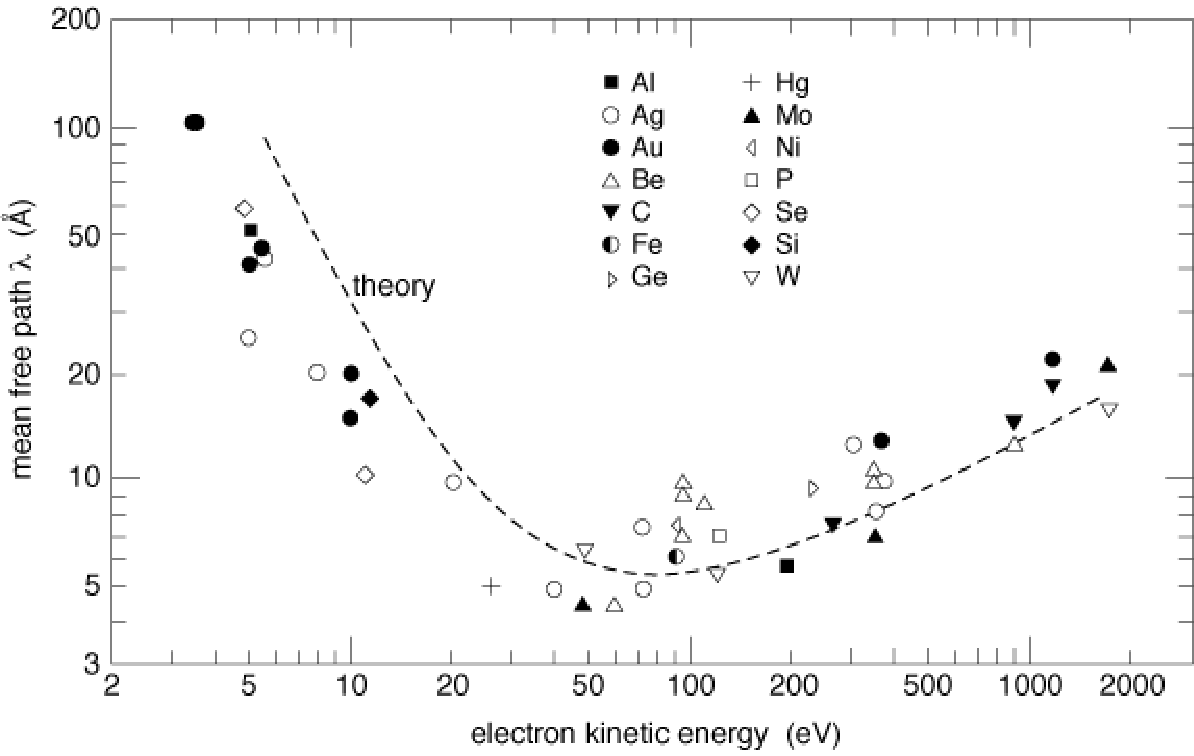
\includegraphics[width=0.6\linewidth]{img/meanfree.pdf}

 \caption{\small Universal curve of solids \cite{zangwill}.  }
        \label{fig:uni}
\end{figure}


\subsection{Photo Emission of an Electron}
When a x-ray photon with an energy $E_\text{ph}=h\nu$ hits an atom, an electron can be emitted, if the energy of the photon is high enough to ionize the atom and provides additional energy for the electron to overcome the work function barrier $\Phi_S$ (in a solid). This general effect is called the Photo-Effect (Nobelprice 1905, Einstein) and its energy balance reads
\eq{h\nu +E(A) =E(A^*)+E_\text{kin} + \Phi_S \;,}{eq:energy}
where $E(A)$ is the energy of the electron level before and $E(A*)$ after ionization. In the experiment, the kinetic energy of the electrons will be analyzed and is given by
\eq{E_\text{kin}= h \nu - E_B -\Phi_S \; ,}{eq:energy2}
where $E_B=E(A)-E(A^*)$ is the binding energy relative to the Fermi Level $E_F$ (cf. fig. \ref{fig:energy}). If the electron spectrograph and the sample are grounded, the work function is actually given by the spectrograph and equation \Formel{eq:energy2} has to be slightly altered
\eq{E_\text{kin}= h \nu - E_B -\Phi_\text{spec} \; .}{eq:energy3}
\begin{figure}
  \centering
   	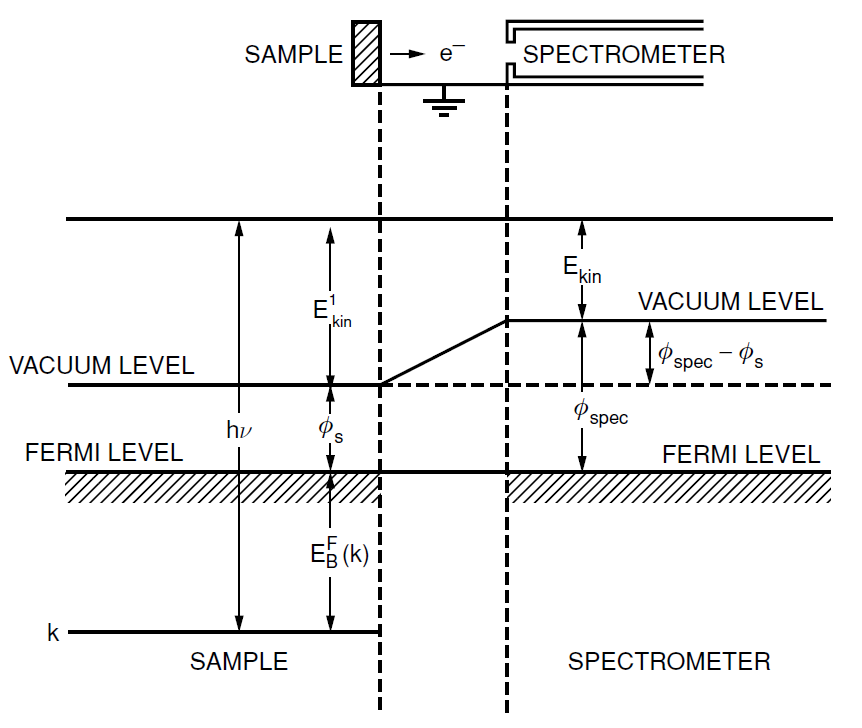
\includegraphics[width=0.6\linewidth]{img/energy.png}
 \caption{\small Energy Diagram for Photo Emission in a Solid. On the right the modification for grounded sample and spectrograph is visualized. Source: \cite{nano} }
        \label{fig:energy}
\end{figure}

\begin{figure}
  \centering
   	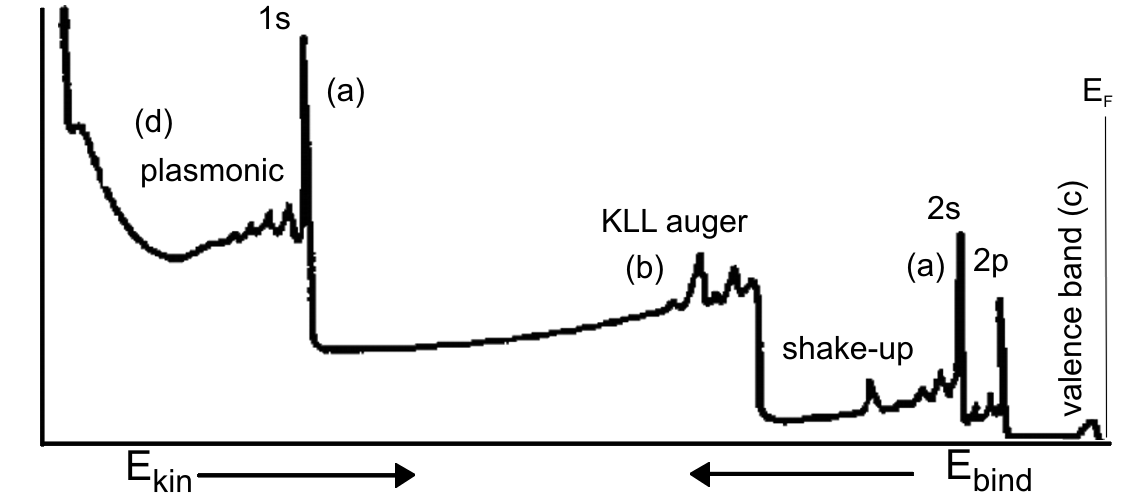
\includegraphics[width=0.6\linewidth]{img/spectrum.png}
 \caption{\small Typical XPS Electron Spectrum. Source : \cite{script} }
        \label{fig:spectrum}
\end{figure}


\subsection{Electron Spectrum}
A typical xps electron spectrum is described in figure \ref{fig:spectrum}. The most significant peaks result from electrons directly emitted from the core levels. The peak with highest kinetic energy is caused by electrons emitted from the valence band, that is close to the Fermi level. Other significant peaks are the Auger peaks, which stem from Auger electrons. In the Auger process a hole created by the ionization of a core level is filled by an electron from a higher shell. The energy, that is set free during this process is passed without radiation to a third electron, which is then ionized and emitted. This last electron is called Auger electron. Its energy is independent of the source used for primary ionization. This feature is useful for determining the Auger peaks within the spectrum, which can be done by comparing two spectra created with different x-ray frequencies.

Other effects, which can be seen in the spectrum are plasmon losses. A plasmon is the pseudo particle of fermi-gas oscillation. These plasmons have characteristic energies, depending on the conduction electron density $n$. 
$$E_p = \hbar \underbrace{\sqrt{\frac{ne^2}{m_e \epsilon_0}}}_{\omega_p}$$
Apart from the more obvious bulk plasmons (three dimensional oscillations in the sample) there are also surface plasmons when a material with positive dielectric constant (vacuum) interfaces with a material of negative dielectric constant. An electron that excites a plasmon looses one of these characteristic energies and is said to have suffered plasmon loss. It is possible, that one electron suffers plasmon loss several times, leading to a series of equally spaced losses with decreasing intensity.
%TODO: shake-up


\subsection{Binding Energy and Multiplet-Structures}
The interaction between the spins of the electrons and their angular momenta, the so called spin-orbit-coupling leads to the splitting of energy niveaus within one shell. In general there are two different types of spin-orbit coupling, distinguished by the dominant coupling effect, which is either the coupling between all electronic angular momenta and all electron spins (LS-Coupling) or between the angular momentum and the spin of each electron separately ($jj$-Coupling). The latter case is relevant in this experiment and its single electron Hamiltonian is given by
\eq{H=a \ve s \cdot \ve l\;,}{hamilton}
where $\ve l$ is the angular momentum of the electron, $\ve s$ the spin and $a$ is the coupling constant. The eigenstates are then characterized by the total angular momentum, which can have the values $(l+\tfrac 1 2)$, $(l - \tfrac 1 2)$ except for the $s$-shell ($l=0$), where no coupling effects between angular momentum and spin can occur. However, it was found by Abragam and experimentally verified, that the degeneracy of the fully filled $s$-state can be lifted by the interaction with another partially filled shell yielding again a two-folded splitting (doublet). This effect is called magnetic spin-spin exchange.

\clearpage
\section{Experimental Set-Up}

\begin{figure} 
 \centering
 \subfloat[][Set-Up]{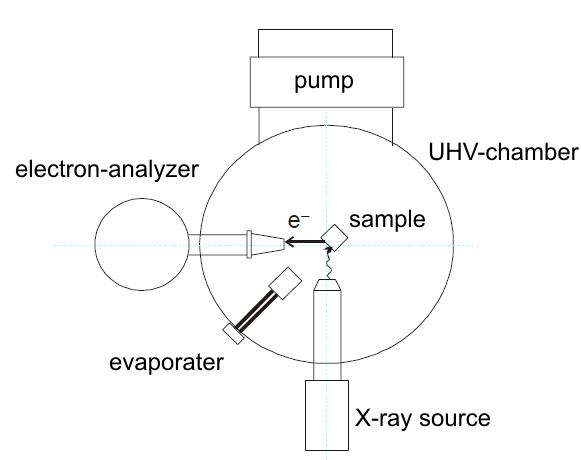
\includegraphics[width=0.45\textwidth]{img/setup.png}}
 \hfill
  \subfloat[][Channeltron]{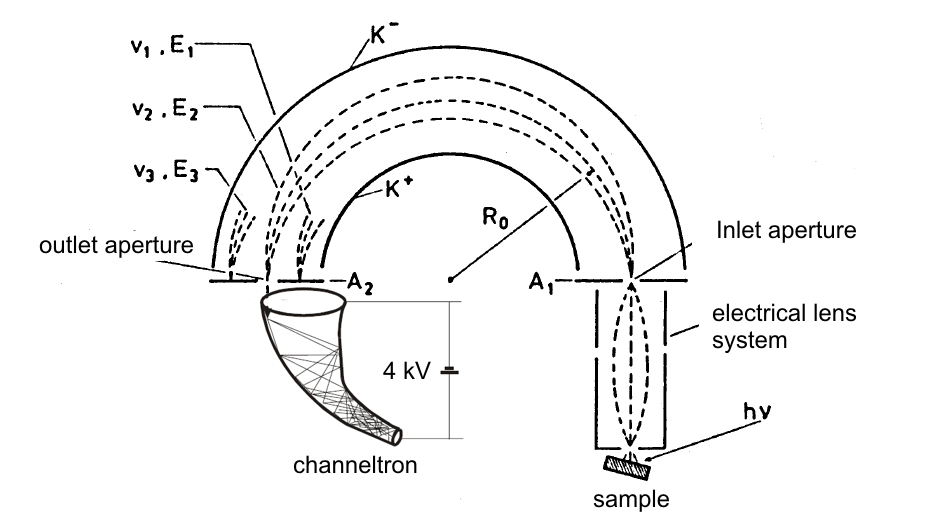
\includegraphics[width=0.45\textwidth]{img/channeltron.png}}

\caption{ \small \textbf{(a)} Schematic Description of the Experimental Set-Up. \textbf{(b)} Channeltron Sources: \cite{script}, \cite{gop} } 
	\label{fig:setup}
\end{figure}
%TODO: channeltron caption.

\subsection{Creation of X-Rays}
%TODO x-rays

\subsection{Ultra High Vacuum (UHV)}
As the electrons used for spectroscopy easily interact with all kind of materials, it is very useful to operate in high vacuum. This is also necessary in order to reduce the rate of adsorption of molecules, which leads to disturbance of the measured spectra. (Ultra) high  vacuum (UHV) can only be achieved by a series of pumps acting within different pressure ranges. The four types used in the experiment are listed in table \ref{tab:pump}.
\begin{wraptable}{r}{0.55\textwidth}
\begin{tabular}{lr}
\toprule
pump & pressure range (Pa)\\
\midrule
\small rotary vane pump & $10^5$ - $10^{-1}$  \\ 
\small turbo molecular pump &  $10^0$  - $10^{-9}$  \\
\small ion getter pump  & $ 10^{-3}$  - $10^{-9}$  \\
\small titan sublimation pump & $10^1$  - $10^{-9}$  \\
\bottomrule
\end{tabular}
\caption{Different pumps and their pressure operating range. \cite{gop} }
\label{tab:pump}
\end{wraptable}

\subsubsection{Rotary vane pump}
The rotary vane pump is a simple mechanical pump, which consists of a cylinder connecting the vacuum cell and the outer space. In the cylinder a vane rotates and thereby shovels the gas to the outside. Springs ensure optimal contact between the vane and the cylinder walls. 



\begin{figure} 
 \centering
\subfloat[][Rotary vane pump]
{        	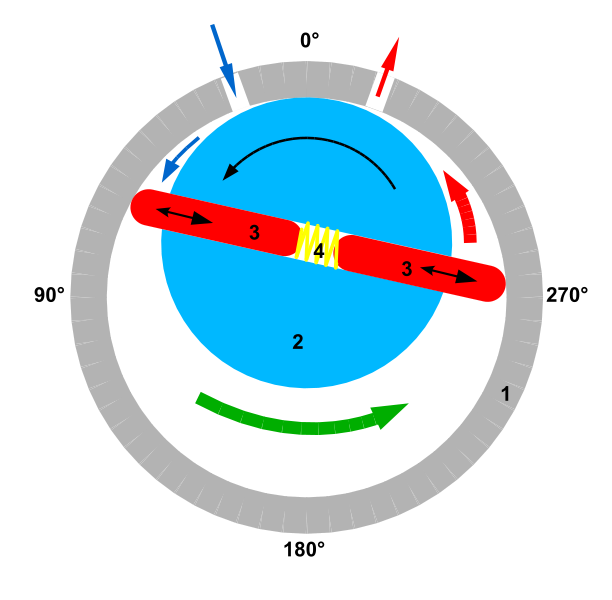
\includegraphics[width=0.45\textwidth]{img/rot.png}}
 \hfill
\subfloat[][Turbomolecular pump]
         { 	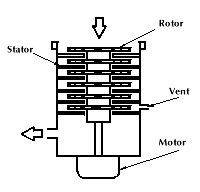
\includegraphics[width=0.45\textwidth]{img/tu.jpg}}
\caption{
\small \textbf{(a)} Rotary vane pump. 1: pump housing, 2: rotor, 3: vanes, 4: spring,  \textbf{(b)} Schematic description of a turbomolecular pump } 
	\label{fig:pump}
\end{figure}






\subsubsection{Turbomolecular pump}
The main features of a turbomolecular pump are the rotating blades (rotors), hitting the molecules very often per unit time, thereby enforcing a velocity distribution within the gas that is not isotropic, but a certain direction is preferred. Within the pump there are other static blades (stators), which act as a kind of filter to the velocity of the molecules in such a way, that molecules with the velocity, that is predominantly created by the rotors, can pass through with a higher probability. These filters act only in one-way, so that the molecules stay on the other side as long as the asymmetric velocity distribution is maintained. 


\subsection{Electron Energy Analyzer}
The electron energy analyzer is the central measurement device, as it performs the resolution of electron numbers with vs. energy. In this experiment a concentric hemispheric capacitor is used as an energy filter (cf. fig. \ref{fig:setup} b). The trajectory of the electron is altered by the electric field of the capacitor, in such a way, that only electrons with a certain range of kinetic energy can pass the analyzer. This pass energy can be chosen by applying appropriate voltage. Before entering the analyzer, the electrons are focussed by an electrical lens system and after they exit the analyzer are detected by a channeltron, that works as an electron multiplier (factor $10^6$ to $10^8$) and produces analog signals, which can be digitalized and processed by a computer. 



\FloatBarrier
 \bibliographystyle{unsrt}
\bibliography{bib}

\end{document}


